\DiaryEntry{Cliffhanger Problem}{2016-09-20}{Stochastic}

We need to distinguish the probability of moving to the right / left \textbf{within one step} which is \(p\) / \(1-p\), respectively and the probability of absorption when started at position \(i\): \(P(abs|i)\). These latter probabilities do not consider how many steps it takes between start and absorption.

We have

\[
P(abs|1) = 1 - p + p P(abs|2)
\]

When we start at one there are two options for absorption: Move to the left directly (with probability \(1-p\)) or move to the right directly (with probability \(p\)) and being absorbed some when later (with probability \(P(abs|2)\)).

The probability for absorption starting at 2 have two parts: Going from 2 to 1 (not necessarily in one step) and going from 1 to 0 (again not necessarily in one step) with probability \(P(abs|1)\). The probability for going from 2 to 1 is the same - the only difference is that everything has been shifted to the right by one position.

Therefore, we have

\[
P(abs|2) = P(abs|1)^2
\]

and inserting this into the first equation, we obtain

\[
P(abs|1) = 1 - p + p P(abs|1)^2
\]

Solving for the absorption probability we obtain the following two solutions

\[
P(abs|1) = 1, P(abs|1) = \frac{1-p}{p}
\]

For the extreme case of \(p=0\) (no movement to the right), we will have \(P(abs|1) = 1\); i.e.~there will always be absorption. For \(p=1/2\) the two solutions yield the same value, namely \(P(abs|1) = 1\), and for the other extreme case of \(p=1\) (no movement to the left), we will have \(P(abs|1) = 0\); i.e.~no absorption.

A plot of the probability \(P(abs|1)\) for different values of \(p\) is shown in the following Figure.

\begin{figure}
\centering
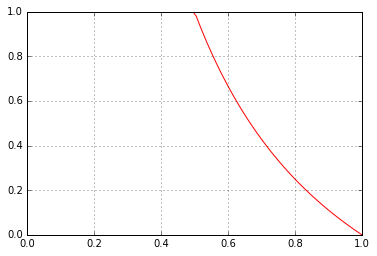
\includegraphics{images/cliffhanger.png}
\end{figure}
